% Options for packages loaded elsewhere
\PassOptionsToPackage{unicode}{hyperref}
\PassOptionsToPackage{hyphens}{url}
\PassOptionsToPackage{dvipsnames,svgnames,x11names}{xcolor}
\documentclass[
]{article}
\usepackage{xcolor}
\usepackage[margin=22mm]{geometry}
\usepackage{amsmath,amssymb}
\setcounter{secnumdepth}{-\maxdimen} % remove section numbering
\usepackage{iftex}
\ifPDFTeX
  \usepackage[T1]{fontenc}
  \usepackage[utf8]{inputenc}
  \usepackage{textcomp} % provide euro and other symbols
\else % if luatex or xetex
  \usepackage{unicode-math} % this also loads fontspec
  \defaultfontfeatures{Scale=MatchLowercase}
  \defaultfontfeatures[\rmfamily]{Ligatures=TeX,Scale=1}
\fi
\usepackage{lmodern}
\ifPDFTeX\else
  % xetex/luatex font selection
\fi
% Use upquote if available, for straight quotes in verbatim environments
\IfFileExists{upquote.sty}{\usepackage{upquote}}{}
\IfFileExists{microtype.sty}{% use microtype if available
  \usepackage[]{microtype}
  \UseMicrotypeSet[protrusion]{basicmath} % disable protrusion for tt fonts
}{}
\makeatletter
\@ifundefined{KOMAClassName}{% if non-KOMA class
  \IfFileExists{parskip.sty}{%
    \usepackage{parskip}
  }{% else
    \setlength{\parindent}{0pt}
    \setlength{\parskip}{6pt plus 2pt minus 1pt}}
}{% if KOMA class
  \KOMAoptions{parskip=half}}
\makeatother
\usepackage{longtable,booktabs,array}
\newcounter{none} % for unnumbered tables
\usepackage{calc} % for calculating minipage widths
% Correct order of tables after \paragraph or \subparagraph
\usepackage{etoolbox}
\makeatletter
\patchcmd\longtable{\par}{\if@noskipsec\mbox{}\fi\par}{}{}
\makeatother
% Allow footnotes in longtable head/foot
\IfFileExists{footnotehyper.sty}{\usepackage{footnotehyper}}{\usepackage{footnote}}
\makesavenoteenv{longtable}
\usepackage{graphicx}
\makeatletter
\newsavebox\pandoc@box
\newcommand*\pandocbounded[1]{% scales image to fit in text height/width
  \sbox\pandoc@box{#1}%
  \Gscale@div\@tempa{\textheight}{\dimexpr\ht\pandoc@box+\dp\pandoc@box\relax}%
  \Gscale@div\@tempb{\linewidth}{\wd\pandoc@box}%
  \ifdim\@tempb\p@<\@tempa\p@\let\@tempa\@tempb\fi% select the smaller of both
  \ifdim\@tempa\p@<\p@\scalebox{\@tempa}{\usebox\pandoc@box}%
  \else\usebox{\pandoc@box}%
  \fi%
}
% Set default figure placement to htbp
\def\fps@figure{htbp}
\makeatother
\setlength{\emergencystretch}{3em} % prevent overfull lines
\providecommand{\tightlist}{%
  \setlength{\itemsep}{0pt}\setlength{\parskip}{0pt}}
\usepackage{bookmark}
\IfFileExists{xurl.sty}{\usepackage{xurl}}{} % add URL line breaks if available
\urlstyle{same}
\hypersetup{
  colorlinks=true,
  linkcolor={Maroon},
  filecolor={Maroon},
  citecolor={Blue},
  urlcolor={Blue},
  pdfcreator={LaTeX via pandoc}}

\author{}
\date{}

\begin{document}

\section{Paper 14: The Choice of Time Direction and the Stage for
Amplitudes --- the Marking Theorem, Derived Z₄ Phases, Inversion
Holonomy, and the Canonical Counting
Theorem}\label{paper-14-the-choice-of-time-direction-and-the-stage-for-amplitudes-the-marking-theorem-derived-zux2084-phases-inversion-holonomy-and-the-canonical-counting-theorem}

\textbf{Author}: Noriaki Kihara \textbf{Date}: June 12, 2026
\textbf{Version}: v1.0 (final; v0.2 incorporated the 5 mandatory points
of the first review {[}major revision{]}, v1.0 the points R1--R6 of the
second review {[}accept with minor conditions{]} --- Proposition 1′
promoted to a proven, range-unlimited statement) \textbf{Series}: Dual
Geometry of Wavelength Space and Frequency Space (Paper 14, sequel to
Papers 1--13)

\begin{center}\rule{0.5\linewidth}{0.5pt}\end{center}

\subsection{Abstract}\label{abstract}

Paper 13 showed that position and time can be read from the axiom
inventory alone. Two questions remained --- \textbf{why does a
particular axis look like time}, and \textbf{where do amplitudes
(complex numbers, phases) come from?} This paper theorematizes both
within the inventory. Main results: (1) \textbf{Choosing a time
direction = choosing a complex structure} (Theorem 1): choosing a time
direction \(u\) inside the quaternions \(\mathbb{H}\) selects the
complex subfield \(C_u\subset\mathbb{H}\), and the polar decomposition
\(q=|q|e^{u\theta}\) yields \textbf{the clock (modulus) and the phase
(argument) simultaneously}. Complex numbers are not an axiom but the
shadow of this choice. A proven companion identity (Proposition 1′, with
a three-line proof, range-unlimited): splitting the dressed vector
\(d_j=2|k_j|+1\) into the Gaussian integers \(v_1=(d_1+id_2)/(1+i)\),
\(v_2=(d_3+id_4)/(1+i)\) gives \(N(v_1)+N(v_2)=2s\) with each \(N(v_j)\)
\textbf{odd} --- the factor \((1+i)\) joins the norm rung to the
odd-Gaussian rung. (2) \textbf{The marking theorem} (Theorem 2):
lattice-compatible quaternion structures number \textbf{exactly 16}, on
which B₄ acts \textbf{transitively} with point stabilizers the
24-element ring-automorphism group (\(384=16\times24\)) --- the real
axis runs over all four axes. The principle ``all axes are symmetric; t
merely appears to have been selected by observation'' becomes a theorem
here. Of the first-order canonical readings defined per marking, the
ones shared by all 16 are \textbf{the norm (R) and the central character
ε (Q)} --- completeness is asserted for that family of functions, not
for arbitrary cell functions. (3) \textbf{Transport phases are derived}
(Theorem 3): the coefficient ratio \(\eta\) between parent line and
daughter cross line is fixed uniquely by the dictionary's trigonometric
identities and \textbf{always lands on \(Z_4=\{1,i,-1,-i\}\)} (zero
exceptions over all paths at s=9/11/13 --- phase assignment rules became
unnecessary). (4) \textbf{The identity of the forced bit} (Theorem 4):
the structure of the channel-consistent aggregate demands exactly one
bit of choice, and its identity is \textbf{not the arrow} (axiom 3;
invariant under time reversal of comparisons) but the \textbf{\(Z_2\)
chain holonomy of canonical inversion \(g\to-g\) = complex conjugation}
--- the system has two independent global \(Z_2\)'s. The diagnostic
quantity here is explicitly the \textbf{channel-consistent sum}, one
particular aggregate, whose measure-theoretic status is adjudicated by
Paper 16; the scope restriction is substantiated by a new check (at s=9
configuration granularity, \(W'_{531}\) is sector-independent, 576=576,
while \(W'_{333}\) retains dependence, 40 vs 16 --- the bit is not an
artifact of the aggregate, but the index-2 formulation is stated at the
channel-consistent level). (5) \textbf{The canonical counting theorem}
(Theorem 5): how to count identical daughters is not a convention ---
configuration reading (state = set) forces \textbf{identical-particle
symmetrization}, uniquely; the treatment of diagonal terms and decay
branches does not affect the amplitude bookkeeping (machine-verified 2×2
separation: ordering × diagonal). What standard theory installs as the
symmetrization postulate appears here as a theorem of set structure ---
and the theorem is \textbf{granularity-robust} (the doubling acts at the
level of per-configuration \(z_K\)). Appendix A collects the general
transport-algebra lemmas (single-axis branch-flip ±i lemma --- 103,168
flips over three shells, zero exceptions; single-sign support; the
charge-like parity theorem; the mirror-flip lemma). \textbf{This paper
does not select an aggregation rule (measure) for path amplitudes} ---
it stops at the definition of η and path sets and their phase algebra
(the measure line is Paper 16). No physical identification is made.

\begin{center}\rule{0.5\linewidth}{0.5pt}\end{center}

\subsection{1. Introduction}\label{introduction}

\subsubsection{1.1 The questions}\label{the-questions}

\textbf{Gauge data held fixed (complete enumeration, same standard as
Paper 13)}: the marking \(u\), per-axis orientations \(Z_2^{4}\), and
the reference fragment (origin). All theorems below are statements about
properties across gauge choices (transitivity; shared invariants).

At the endpoint of Paper 13 the four axes were fully symmetric
(interchangeable, including R and Q) and t was a derived quantity. Then:
why does some direction look like ``time'' to an observer? And since
complex numbers exist nowhere among the axioms of Papers 5--12, while
the record readout (branch channels, Paper 13, Theorem 3) handles
complex coefficients --- \textbf{where did i come from?} The answer:
both are two faces of one and the same choice --- \textbf{time direction
= complex structure} --- whose freedom, invariants, and the
exactly-one-bit remainder can all be theorematized.

\subsubsection{1.2 What is not claimed}\label{what-is-not-claimed}

\begin{enumerate}
\def\labelenumi{(\roman{enumi})}
\tightlist
\item
  \textbf{This paper does not select an aggregation rule (measure) for
  path amplitudes.} It theorematizes the raw material (η, path sets,
  phase algebra); how they are bundled into probabilities is the
  business of the ongoing measure line (Paper 16), and no result here
  depends on that outcome. (ii) The full continuous phase U(1) is not
  claimed --- what is derived is \(Z_4\), and
  \(Z_4\hookrightarrow U(1)\) is an inclusion. (iii) No physical
  identification is made. References to standard-theory counterparts are
  confined to the abstract and to the form ``what standard theory
  installs as \ldots{}'' in theorem statements; interpretive
  correspondences are quarantined with labels.
\end{enumerate}

\subsection{2. Choosing a time direction = choosing a complex
structure}\label{choosing-a-time-direction-choosing-a-complex-structure}

The algebraic stage of the four axes is the quaternions \(\mathbb{H}\)
(the \{1,2,4,8\} series of Paper 11).

\textbf{Standard fact (mathematics)}: for a unit pure imaginary \(u\),
\(C_u=\mathbb{R}\oplus\mathbb{R}u\subset\mathbb{H}\) is a subfield
isomorphic to \(\mathbb{C}\), and the polar decomposition
\(q=|q|e^{u\theta}\) exists --- a standard fact about quaternions, not
subject to verification.

\begin{quote}
\textbf{Theorem 1 (model-specific content)}: the system's choice of time
direction is realized as the choice of \(C_u\); the modulus coincides
with the norm clock of Paper 13, Theorem 5, and the argument with the
phase (where the η of §4 lives) --- \textbf{clock and phase are obtained
simultaneously from one choice}. Complex numbers and phases are products
of this choice, not axioms.
\end{quote}

\begin{quote}
\textbf{Proposition 1′ (junction with the amplitude rung --- proven,
range-unlimited)}: for any cell \(k\in\mathbb{Z}^4\), split the dressed
vector \(d_j=2|k_j|+1\) into two pairs and set the Gaussian integers
\(v_1=(d_1+id_2)/(1+i)\), \(v_2=(d_3+id_4)/(1+i)\). Then \(v_1,v_2\) are
Gaussian integers, \(N(v_1)+N(v_2)=2s\), and each \(N(v_j)\) is
\textbf{odd}.

\textbf{Proof} (three lines; second review R2, claude.ai): \(d_j\) odd ⟹
\(d_1+d_2\) even ⟹ \((1+i)\mid(d_1+id_2)\) (divisibility).
\(N(v_1)+N(v_2)=(\sum d_j^2)/2=2s\) (since \(s=(\sum d_j^2)/4\)).
\(d_j^2\equiv1\ (\mathrm{mod}\ 8)\) ⟹
\(N(v_j)=(d_a^2+d_b^2)/2\equiv1\ (\mathrm{mod}\ 4)\), hence odd. ∎
\end{quote}

Machine confirmation (②): 6561/6561 over \(k\in\{-4..4\}^4\). The factor
\((1+i)\) joins the norm rung (even \(2s\)) to the odd-Gaussian-norm
rung.

\subsection{3. The marking theorem --- the all-axes-symmetric principle
as a
theorem}\label{the-marking-theorem-the-all-axes-symmetric-principle-as-a-theorem}

\begin{quote}
\textbf{Theorem 2 (marking theorem)}: lattice-compatible quaternion
structures (markings) number \textbf{exactly 16}, and B₄ (384 elements)
acts on them \textbf{transitively} --- each point stabilizer is the
ring-automorphism group (24 elements), \(384=16\times24\) (first review
\#1 corrected the earlier ``simply transitive'': simple transitivity
would require \(|G|=|X|\)). \textbf{Enumeration (reproducible
procedure)}: transport the standard quaternion product by all 384
elements of B₄ and deduplicate the resulting multiplication tables; 16
distinct structures remain (four with the real axis on each of the four
axes; script E1). Moreover (i) the real axis runs over all four axes
(E2); (ii) \textbf{of the first-order canonical readings defined per
marking (real part, modulus, central character), those shared by all 16
markings (= completely B₄-invariant) are exactly the norm \(s\) (→R) and
\(\varepsilon\) (→Q)} (E3; ``only'' is completeness with respect to this
family of functions, not arbitrary cell functions --- quantified per
first review \#2).
\end{quote}

Consequence: which axis is time is \textbf{gauge} (chart choice); R and
Q alone are viewpoint-independent ledgers --- the constraint surface
\(\Sigma=\{R^2=s,\ Q=\varepsilon\}\) of Paper 15 is the coordinate
expression of this theorem. The complete gauge data of a chart is the
marking (16) plus the per-axis orientations (\(Z_2^{4}\)).

\subsection{4. The derivation of transport phases --- assignment rules
vanish}\label{the-derivation-of-transport-phases-assignment-rules-vanish}

When the parent's identity line persists into the daughters' cross lines
across a decay (record continuity, Paper 12), the coefficient ratio

\[
\eta=\frac{C_{\rm cross}/|C_{\rm cross}|}{C_{\rm parent}/|C_{\rm parent}|}
\]

is fixed uniquely by the dictionary (the trigonometric identities of
cos/sin) alone.

\begin{quote}
\textbf{Theorem 3 (Z₄ quantization)}: on every two-stage custody path,
\(\eta\in Z_4=\{1,i,-1,-i\}\) (including the 196 paths at s=9;
\textbf{zero exceptions} through s=11/13; Fig. 1).
\end{quote}

The provisional phase-assignment rules of earlier stages thereby became
\textbf{unnecessary} --- phase is a derived object, not a rule.
\(Z_4\hookrightarrow U(1)\): the continuous phase is the inclusion
target; only the inclusion is claimed.

\subsection{5. The forced bit = inversion chain
holonomy}\label{the-forced-bit-inversion-chain-holonomy}

\textbf{Terminology note (R4)}: the ``classes A/B'' of this section are
holonomy classes (relative parities of link orientations) and are
\textbf{distinct} from the mirror pairs A/B (parents \(\pm m\)) of the
measure line (Paper 16) --- beware of confusion when reading both.

\textbf{The diagnostic made explicit (first review \#4)}: the \(z\) of
this section is the \textbf{channel-consistent sum} (the sum of η over
all custody paths within a channel) --- one particular aggregate, whose
measure-theoretic status (including its divergence from configuration
granularity W′) is adjudicated by Paper 16. The theorems of this section
are stated as \textbf{bookkeeping properties of this aggregate} and
contain no measure claim. One piece of substance behind the scope
restriction (added during this review): at s=9 configuration
granularity, \(W'_{531}\) becomes \textbf{sector-independent} (576=576)
while \(W'_{333}\) retains dependence (40 vs 16) --- the holonomy bit is
not an artifact of the aggregate choice, but the ``index 2'' formulation
below is at the channel-consistent level.

The structure of this aggregate (the exact vanishing of the fully
covariant reduction, and the fact that the \(|z|^2\)-preserving subgroup
of B₄ has \textbf{index 2} --- Appendix A-4) demands exactly \textbf{one
bit} of choice. Its identification (Fig. 3):

\begin{quote}
\textbf{Theorem 4 (bit ≠ arrow)}: time-reversing the comparisons (full
conjugation) leaves \(|z|^2\) \textbf{invariant} --- the forced bit is
\textbf{not} the arrow of axiom 3. The link-orientation group
\(Z_2\times Z_2\) (the four \((o_1,o_2)\)) has been checked
\textbf{exhaustively}: a single-link flip toggles the class, a double
flip restores it (per \#5: the exhaustiveness is over the orientation
group; conjugation and the mirror parent are additional samples). The
identity of the bit is therefore the \textbf{\(Z_2\) chain holonomy of
canonical inversion \(g\to-g\) (complex conjugation on the dual side)}.
\end{quote}

The system's global \(Z_2\)'s are \textbf{two} (arrow; inversion
holonomy), machine-verified to be independent. Inversion is the
canonical structure every abelian group carries automatically --- not an
axiom; the inventory's ``comes for free'' part is where the final bit
lives.

\subsection{6. The canonical counting theorem --- symmetrization is not
a
postulate}\label{the-canonical-counting-theorem-symmetrization-is-not-a-postulate}

How to count identical (same-shell) daughter pairs looks at first like a
choice of convention. However:

\begin{quote}
\textbf{Theorem 5 (canonical counting)}: configuration reading (the
state is the \textbf{set} of occupied cells) forces \textbf{unordered
counting = symmetrization} of identical daughters. Ordered
(distinguishable) counting double-counts identical physical
configurations and inflates the equal-shell second-stage amplitude by a
factor 2. Meanwhile, \textbf{the treatment of diagonal terms (double
occupancy) and decay branches does not affect the amplitude bookkeeping}
(machine-verified 2×2 separation = ordering (unordered/ordered) ×
diagonal (excluded/included); same axis names as the legend of Fig. 2).
\end{quote}

What standard theory installs as the \textbf{symmetrization postulate}
(identical particles are not counted separately) appears here as a
theorem of set structure. \textbf{Granularity audit} (the same audit as
\#4): the ordered-counting inflation acts at the level of
per-configuration amplitudes \(z_K\), so the theorem operates
identically under both channel-consistent (W) and
configuration-granularity (W′) aggregation ---
\textbf{granularity-robust}, independent of the measure line's
adjudication. Note: the theorem fixes the amplitude bookkeeping; it does
not select the rule reading those values as probabilities (§1.2).

\subsection{7. (Conjecture) The number ring of
amplitudes}\label{conjecture-the-number-ring-of-amplitudes}

From the derived \(Z_4\) phases and the dyadic coefficient support
(powers of \(\sqrt2\)), we conjecture that \textbf{amplitudes take
values in the Gaussian integers \(\mathbb{Z}[i]\) (localized at
\((1+i)\))}. Proposition 1′'s \((1+i)\) junction and the ±i lemma family
of Appendix A are consistent with the conjecture, but the proof is open;
it is registered \textbf{as a conjecture}.

\subsection{8. Honest limits}\label{honest-limits}

\begin{enumerate}
\def\labelenumi{\arabic{enumi}.}
\tightlist
\item
  \textbf{No measure is selected} (§1.2 restated) --- sector realization
  (which holonomy class is observed), aggregation rules, and the
  channel-specific cancellation theorems belong to the ongoing measure
  line and are not housed here.
\item
  The exhaustiveness of Theorem 3 is s=9/11/13. General-s algebraic
  proofs rest partly on the lemma family of Appendix A (the general
  proof of single-sign support remains open).
\item
  The identity in Theorem 5 is verified within single-shape shells ---
  boundary cases of mixed-shape shells are unexamined.
\item
  Continuous phases and amplitudes have the status of inclusion and
  conjecture (§4, §7).
\item
  No physical identification is made.
\end{enumerate}

\subsection{Figures}\label{figures}

\begin{itemize}
\tightlist
\item
  \textbf{Figure 1} (\texttt{paper14\_fig1\_eta\_z4.png}): the transport
  phase η on the complex plane --- all 196 paths (s=9) land exactly on
  Z₄ (531: 24/44/56/36; 333: 6/10/12/8; \(\eta^2=\pm1\) at 80/80 and
  18/18)
\end{itemize}

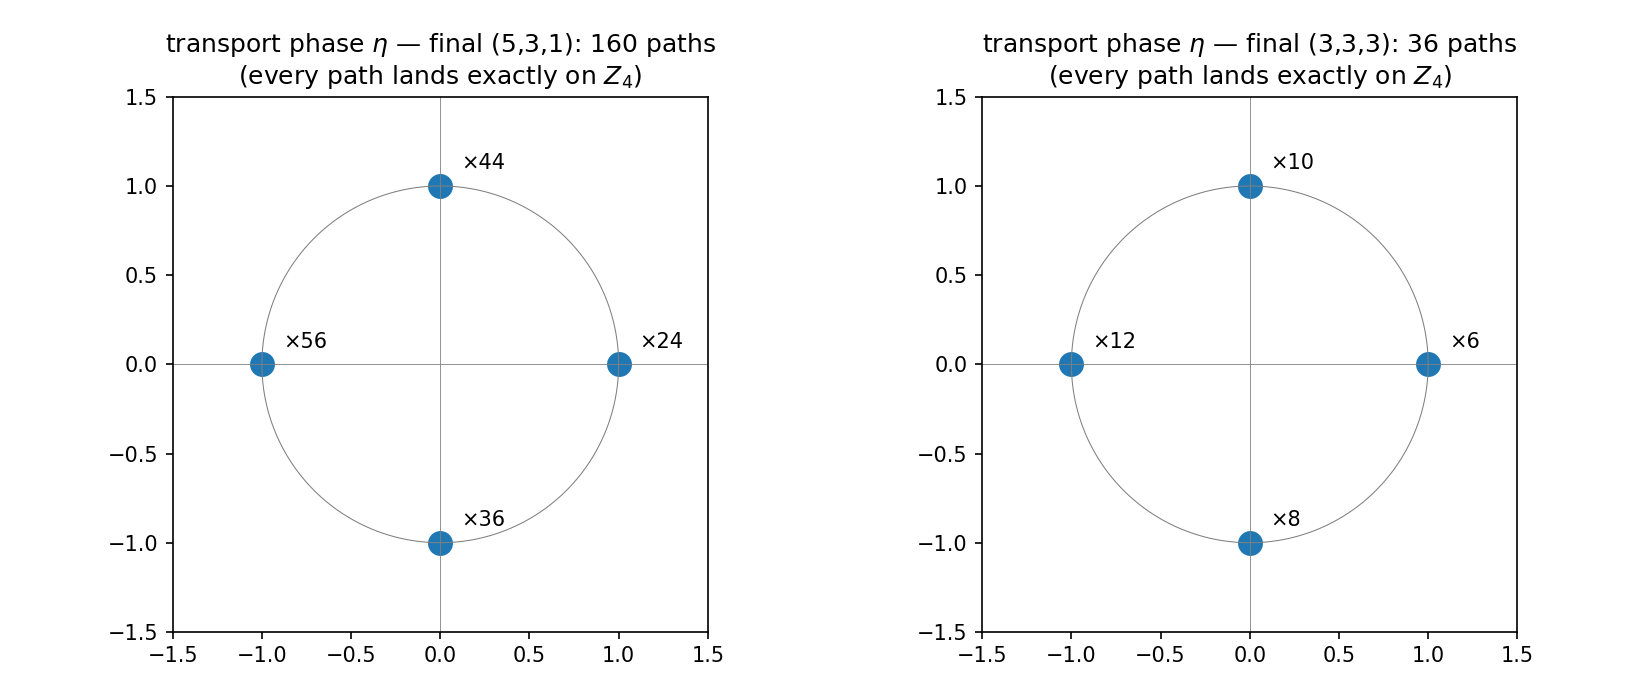
\includegraphics[width=1\linewidth,height=\textheight,keepaspectratio]{paper14_fig1_eta_z4.png}
- \textbf{Figure 2} (\texttt{paper14\_fig2\_convention.png}): the 2×2
separation of canonical counting --- the diagonal is irrelevant (40=40,
160=160); only ordering doubles the amplitude

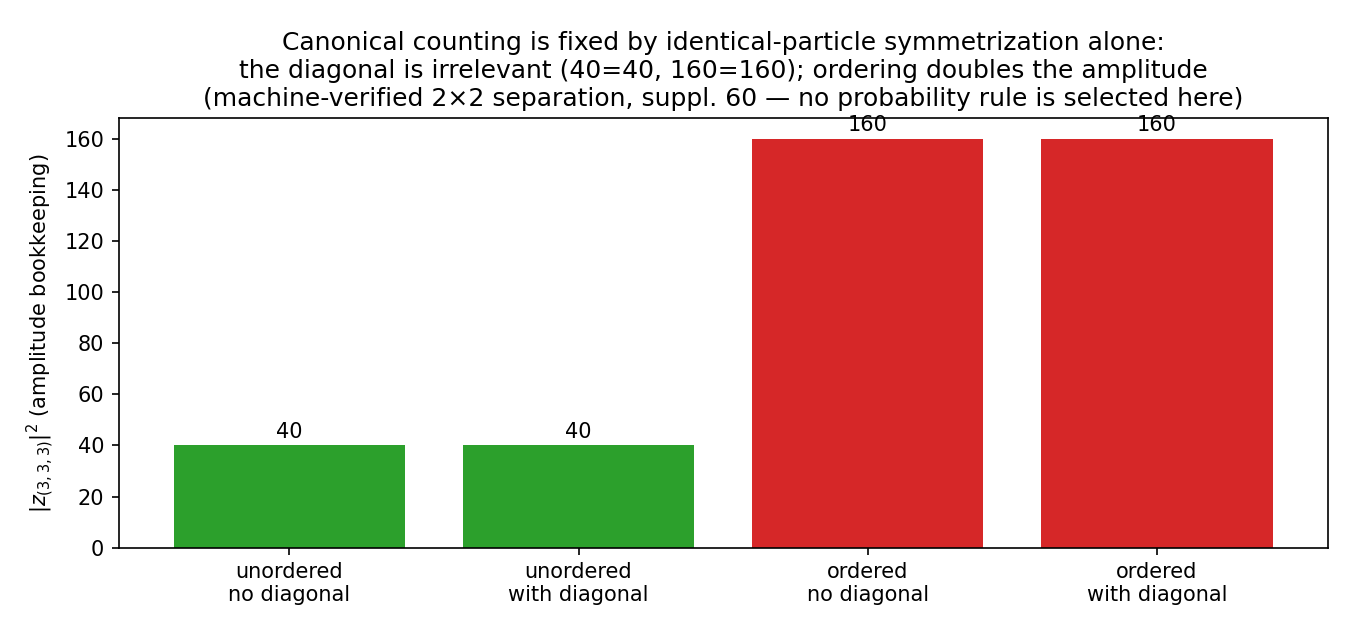
\includegraphics[width=1\linewidth,height=\textheight,keepaspectratio]{paper14_fig2_convention.png}
- \textbf{Figure 3} (\texttt{paper14\_fig3\_holonomy.png}):
identification of the bit --- invariant under T1 (arrow reversal);
single-link flips toggle A↔B; double flip restores

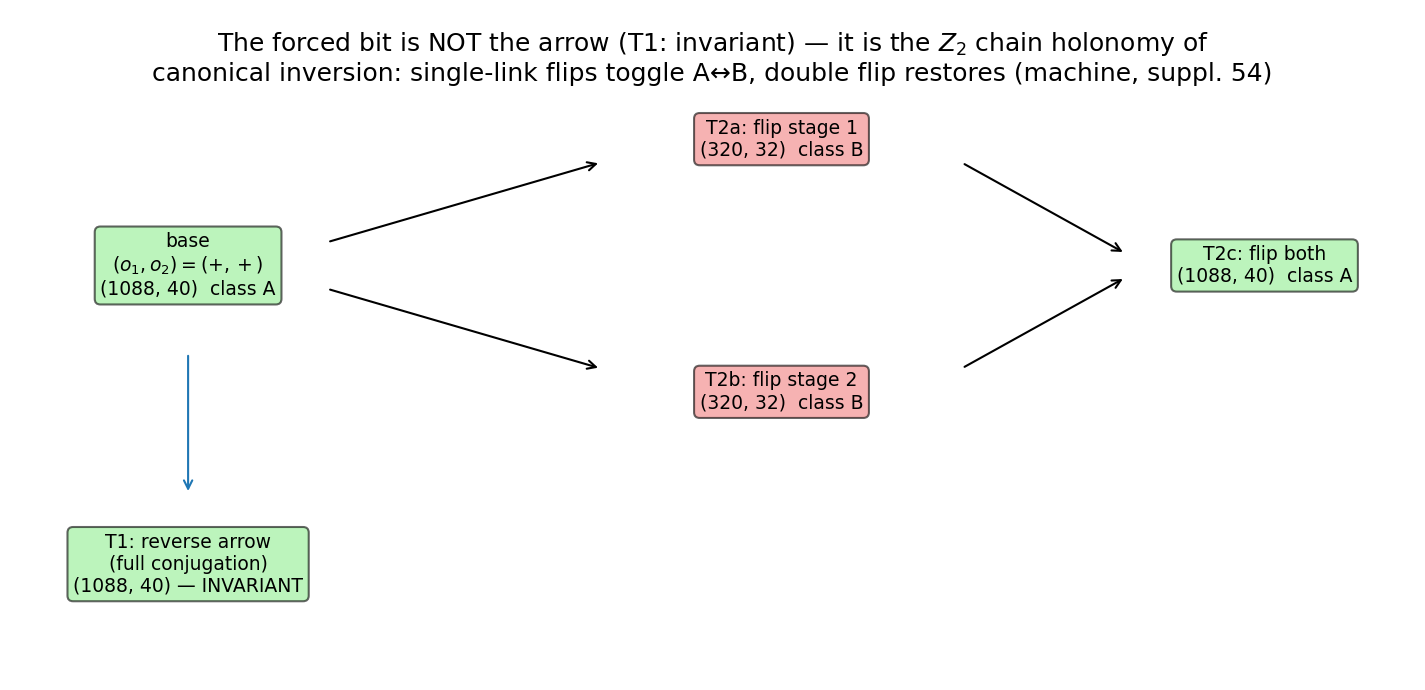
\includegraphics[width=1\linewidth,height=\textheight,keepaspectratio]{paper14_fig3_holonomy.png}

All figures are exact computations or presentations of machine-verified
values (no schematics).

\subsection{Appendix A: General transport-algebra lemmas (with
exhaustive
verification)}\label{appendix-a-general-transport-algebra-lemmas-with-exhaustive-verification}

{\def\LTcaptype{none} % do not increment counter
\begin{longtable}[]{@{}
  >{\raggedright\arraybackslash}p{(\linewidth - 4\tabcolsep) * \real{0.3333}}
  >{\raggedright\arraybackslash}p{(\linewidth - 4\tabcolsep) * \real{0.3333}}
  >{\raggedright\arraybackslash}p{(\linewidth - 4\tabcolsep) * \real{0.3333}}@{}}
\toprule\noalign{}
\begin{minipage}[b]{\linewidth}\raggedright
Lemma
\end{minipage} & \begin{minipage}[b]{\linewidth}\raggedright
Content
\end{minipage} & \begin{minipage}[b]{\linewidth}\raggedright
Verification
\end{minipage} \\
\midrule\noalign{}
\endhead
\bottomrule\noalign{}
\endlastfoot
A-1 single-axis branch flip & a single-axis branch flip (cos↔sin)
multiplies a nonzero transport coefficient by exactly ±i and preserves
nonvanishing & exhaustive at s=9/11/13: \textbf{103,168 flips, 0
annihilations, 0 counterexamples} \\
A-2 single-sign support & contributing cross sums are single-signed per
axis & 55,267 coefficients, exhaustive \\
A-3 charge-like parity & \(C\neq0\Rightarrow\varepsilon\)
multiplicatively conserved (one-line parity arithmetic on the support).
\textbf{As a general lemma this table is canonical; Theorem 8 of Paper
15 is its selection-rule expression} & 118,944 paths + control
39.2\%→0 \\
A-4 index 2 & the \(|z|^2\)-preserving subgroup of B₄ has index 2
(192/384) & exhaustive \\
A-5 mirror flip & reflection to the mirror parent gives
\(\eta_B/\eta_A=-i(-1)^{\sigma_0}\) (\(\sigma_0\) = axis-0 sin-branch
count of the first-stage daughter pair) & m=2: 10/10; m=3: 384/384
(including coincidence of path sets) \\
\end{longtable}
}

These are algebra of transport coefficients \textbf{independent of
channels and aggregation rules}. The channel-specific cancellation
theorems (η² equidistribution, A1, B2, \ldots) concern the
measure-theoretic status of channel-consistent sums and are not housed
in this paper (the measure line --- §8-1).

\subsection{Appendix B: Verification summary (labels: ① true by
construction / ② theorem + confirmation / ③ check that could have
failed)}\label{appendix-b-verification-summary-labels-ux2460-true-by-construction-ux2461-theorem-confirmation-ux2462-check-that-could-have-failed}

{\def\LTcaptype{none} % do not increment counter
\begin{longtable}[]{@{}
  >{\raggedright\arraybackslash}p{(\linewidth - 8\tabcolsep) * \real{0.2000}}
  >{\raggedright\arraybackslash}p{(\linewidth - 8\tabcolsep) * \real{0.2000}}
  >{\raggedright\arraybackslash}p{(\linewidth - 8\tabcolsep) * \real{0.2000}}
  >{\raggedright\arraybackslash}p{(\linewidth - 8\tabcolsep) * \real{0.2000}}
  >{\raggedright\arraybackslash}p{(\linewidth - 8\tabcolsep) * \real{0.2000}}@{}}
\toprule\noalign{}
\begin{minipage}[b]{\linewidth}\raggedright
Claim
\end{minipage} & \begin{minipage}[b]{\linewidth}\raggedright
Label
\end{minipage} & \begin{minipage}[b]{\linewidth}\raggedright
Verification
\end{minipage} & \begin{minipage}[b]{\linewidth}\raggedright
Method
\end{minipage} & \begin{minipage}[b]{\linewidth}\raggedright
Script
\end{minipage} \\
\midrule\noalign{}
\endhead
\bottomrule\noalign{}
\endlastfoot
Theorem 2, markings (enumeration, transitivity) & ③ & dedup of 384
transported tables & exhaustive &
supplement50\_marking\_orbit\_check.py \\
Theorem 2(ii), shared readings & ③ & invariance under all 384 &
exhaustive & same (E3) \\
Proposition 1′, identity and oddness & \textbf{② (three-line proof)} &
6561 cells & in-range confirmation &
supplement49\_quaternion\_split\_check.py \\
Theorem 3, Z₄ quantization & ③ & all paths s=9/11/13 & exhaustive &
supplement51\_phase\_custody\_derivation.py,
supplement56\_s11\_s13\_robustness.py \\
Theorem 4, T1/T2 & ③ & orientation group \(Z_2\times Z_2\) = 4 elements
& exhaustive (orientation group) + samples &
supplement54\_bit\_identification\_tests.py \\
Theorem 4, scope note (W′ sector dependence) & ③ & s=9, both sectors &
exhaustive & paper14\_v02\_wprime\_check.py \\
Theorem 5, 2×2 separation (ordering × diagonal) & ③ & 4 conventions × 2
channels & exhaustive & supplement58\_canonical\_convention.py, suppl.
60 verification \\
Lemmas A-1/A-2 & ③ (general-s proof queued) & 103,168 / 55,267 &
exhaustive & supplement70\_lemma\_and\_4tie.py,
supplement71\_bg\_lemma\_m3.py \\
Lemma A-5 & ② (three-line arithmetic) & 394 paths & exhaustive
confirmation & supplement81\_mirror\_lemma\_check.py \\
\end{longtable}
}

\begin{center}\rule{0.5\linewidth}{0.5pt}\end{center}

\textbf{Acknowledgments / history}: verification was carried out under
the two-party independent verification protocol of Claude Code (local
machine verification) and claude.ai (independent re-computation). Source
material: Supplements 49--54, 56--60, 70, 71, 80 (Lemma A-5: derivation
claude.ai, verification Claude Code), 81 (June 12, 2026). v0.2: 5
mandatory points of the first review. v1.0: points R1--R6 of the second
review --- transcription of the three-line proof of Proposition 1′ (by
claude.ai), label column, W′ verification script, sector terminology
note, batch processing of first-round recommendations.

No physical identification is made.

\end{document}
